\documentclass[14pt, a4paper]{extarticle}

\usepackage{my_GOST}
\usepackage{hyperref}
\usepackage{listings}
\usepackage{array}
\usepackage{caption}
\hypersetup{
	pdftex,
	colorlinks = true,
	linkcolor = black,
	filecolor = magenta,
	citecolor = green,      
	urlcolor = cyan,
}

% к таблице и листингу подпись сверху, перед каждым иллюстративным материалом анонсировать
% написатьт в квадратных скобках к рекурсии комментарием что это метод и понятно почему вызываем его снова
\definecolor{mylightgray}{RGB}{240,240,240}
\definecolor{mygreen}{rgb}{0,0.6,0}
\definecolor{mygray}{rgb}{0.5,0.5,0.5}
\definecolor{mymauve}{rgb}{0.58,0,0.82}

\lstset{
	backgroundcolor=\color{mylightgray},rulecolor=\color{red},  % choose the background color; you must add \usepackage{color} or \usepackage{xcolor}; should come as last argument
	basicstyle=\footnotesize\ttfamily,        % the size of the fonts that are used for the code
	breakatwhitespace=false,         % sets if automatic breaks should only happen at whitespace
	breaklines=true,                 % sets automatic line breaking
	captionpos=t,                    % sets the caption-position to bottom
	commentstyle=\color{mygreen},    % comment style
	extendedchars=false,              % lets you use non-ASCII characters; for 8-bits encodings only, does not work with UTF-8
	firstnumber=0,                % start line enumeration with line 1000
	frame=shadowbox,
	%rulesepcolor=\color{green},	                   % adds a frame around the code
	keepspaces=true,                 % keeps spaces in text, useful for keeping indentation of code (possibly needs columns=flexible)
	keywordstyle=\color{blue}\textbf,       % keyword style
	language=C++,                 % the language of the code
	morekeywords={*,...},            % if you want to add more keywords to the set
	numbers=left,                    % where to put the line-numbers; possible values are (none, left, right)
	numbersep=5pt,                   % how far the line-numbers are from the code
	numberstyle=\scriptsize\color{mygray}, % the style that is used for the line-numbers
	rulecolor=\color{black},         % if not set, the frame-color may be changed on line-breaks within not-black text (e.g. comments (green here))
	showspaces=false,                % show spaces everywhere adding particular underscores; it overrides 'showstringspaces'
	showstringspaces=false,          % underline spaces within strings only
	showtabs=false,                  % show tabs within strings adding particular underscores
	stepnumber=1,                    % the step between two line-numbers. If it's 1, each line will be numbered
	stringstyle=\color{mymauve},     % string literal style
	tabsize=4,	                   % sets default tabsize to 2 spaces
	title=\lstname                   % show the filename of files included with \lstinputlisting; also try caption instead of title
}
\usepackage{YATPR}

\usepackage[utf8]{inputenc}
\usepackage{amsmath}
\usepackage{float}

\begin{document}
\begin{titlepage}
	\newgeometry{pdftex, left=2cm, right=2cm, top=2.5cm, bottom=2.5cm}
	\fontsize{12pt}{12pt}\selectfont
	\noindent \begin{minipage}{0.15\textwidth}
		
\includegraphics[width=\linewidth]{pictures/b_logo.jpg}
	\end{minipage}
	\noindent\begin{minipage}{0.9\textwidth}\centering
		\textbf{Министерство науки и высшего образования Российской Федерации}\\
		\textbf{Федеральное государственное бюджетное образовательное учреждение высшего образования}\\
		\textbf{«Московский государственный технический университет имени Н.Э.~Баумана}\\
		\textbf{(национальный исследовательский университет)»}\\
		\textbf{(МГТУ им. Н.Э.~Баумана)}
	\end{minipage}
	
	\noindent\rule{18cm}{3pt}
	\newline\newline
	\noindent ФАКУЛЬТЕТ $\underline{\text{«Информатика и системы управления»}}$ \newline\newline
	\noindent КАФЕДРА $\underline{\text{«Программное обеспечение ЭВМ и информационные технологии»}}$\newline\newline\newline\newline\newline\newline\newline
	
	
	\begin{center}
		\Large\textbf{Отчет по лабораторной работе №5}\newline
	\end{center}
	
	\noindent\textbf{Название} $\underline{\text{~Моделирование работы информационного центра~~~~~~~~~}}$\newline\newline\newline
	\noindent\textbf{Дисциплина} $\underline{\text{~Моделирование~~~~~~~~}}$\newline\newline
	\noindent\textbf{Студент} $\underline{\text{Зайцева А. А.~~~~~~~~~~~~~~~~~~~~~~~~~~~~~~~~~~~~~~~~~}}$\newline\newline
	\noindent\textbf{Группа} $\underline{\text{ИУ7-72Б~~~~~~~~~~~~~~~~~~~~~~~~~~~~~~~~~~~~~~~~~~~~}}$\newline\newline
	\noindent\textbf{Оценка (баллы)} $\underline{\text{~~~~~~~~~~~~~~~~~~~~~~~~~~~~~~~~~~~~~~~~~~~~~~~~~}}$\newline\newline
	\noindent\textbf{Преподаватель}$\underline{\text{~Рудаков И. В.~~~~~~~~~~}}$\newline
	
	\begin{center}
		\vfill
		Москва~---~\the\year
		~г.
	\end{center}
 \restoregeometry
\end{titlepage}


\setcounter{page}{2}

\section{Задание}

Написать программу, которая генерирует алгоритмическим способом и получает табличным способом случайные последовательности одноразрядных, двухразрядных и трехразрядных целых чисел.

Разработать количественный критерий оценки случайности последовательности чисел. Для каждой полученной последовательности вычислить и вывести значение критерия.

Предусмотреть возможность ввода последовательности чисел и оценки их случайности с помощью критерия.


\section{Теоретические сведения}

\subsection{Способы получения случайных чисел}

На практике наиболее распространены 3 способа получения случайных чисел.

\textbf{Аппаратный способ}

При использовании аппаратного способа случайные числа вырабатываются специальной электронной приставкой (генератором случайных чисел). Реализация данного способа не требует дополнительных вычислений, необходима только одна операция -- обращение к вычислительному устройству. 

В качестве физического эффекта, лежащего в основе генерации случайных чисел, может использоваться, например, шум в электронных приборах.  Для генерации необходимы источник шума, ключевая схема, формирователь импульсов и пересчетная схема.

%Аппаратные генераторы случайных чисел – это устройства, использующие для создания случайных чисел замеры параметров некоторых физических процессов. Как правило, аппаратный генератор случайных чисел состоит из источника энтропии и устройства, преобразующего значения, полученные с источника энтропии, в нужный формат.


\textbf{Табличный способ}

Случайные числа берутся из заранее подготовленной таблицы, которая находится во внешней или оперативной памяти. Числа в таблице проверены на случайность и некоррелированы.



\textbf{Алгоритмический способ}

Алгоритмический способ основан на использовании специальных алгоритмов. К таким алгоритмам, например, относятся следующие:

\begin{itemize}
	\item алгоритм Фон-Неймана (метод серединных квадратов);
	\item метод перемешивания (сдвигов);
	\item линейный конгруэнтный генератор;
	\item вихрь Мерсенна.
\end{itemize}



\subsection{Критерий оценки случайности последовательности}

Для количественного отображения того, насколько <<случайной>> является последовательность, было решено рассматривать разницы значений соседних элементов последовательности. 

Пусть дана последовательность $X$ из $n$ целых чисел из некоторого интервала $[x_{min}; x_{max}]$:
\begin{equation}
	\begin{gathered}
		x = \left(x_1, ..., x_n\right), \quad \text{где} \\
		x_{min} \leq x_i \leq x_{max}, \forall i \in \{1, ..., n\}.
	\end{gathered}
\end{equation}

По ним вычисляется последовательность $D$ разностей соседних элементов:
\begin{equation}
	\begin{gathered}
	D = \left(d_1, ..., d_k\right), \quad \text{где} \\
	k = \left[\frac{n}{2}\right],\\
	d_i = x_{2i + 1} - x_{2i}.
	\end{gathered}
\end{equation}

Всевозможные разности целых чисел из интервала $[x_{min}; x_{max}]$ можно представить в виде последовательности из $s=2\left(x_{max} - x_{min}\right) - 1$ целых чисел $DP$:
\begin{equation}
	\begin{gathered}
		DP = \left(x_{min} - x_{max} + 1, x_{min} - x_{max} + 2, ..., x_{max} - x_{min}\right).
	\end{gathered}
\end{equation}

Вероятность $p_i$ того, что разность соседних элементов равна числу $dp_i \in DP$, можно вычислить по следующей формуле:

\begin{equation}
	\begin{gathered}
		p_i = P\left(\text{dif} = dp_i\right) = \frac{x_{max} - x_{min} - \lvert dp_i \lvert}{(x_{max} - x_{min})^2}
	\end{gathered}
\end{equation}

Тогда, подсчитав для каждой теоретически возможной разности $dp_i \in DP$ количество ее вхождений $y_i$ в полученную последовательность $D$, можно рассчитать статистику $\chi^2$ по следующей формуле:
\begin{equation}
	V = \frac{1}{k} \sum_{i = 1}^{s} \frac{y_{i}^2}{p_i} - k.
\end{equation}
 
Затем с помощью этого количественного критерия V дается качественная оценка <<случайности>> последовательности. С помощью таблицы процентных точек распределения $\chi^2$ с количеством степеней свободы $v=x_{max} - x_{min}$, определяется, между какими точками находится вычисленное значение V. Если оно оказывается между 5\% и 95\% точками, то делается вывод, что числа исходной последовательности $X$ -- случайные; если оно оказывается левее 1\% точки или правее 99\% точки, то последовательность $X$ признается не случайной; в ином случае последовательность $X$ характеризуется как <<подозрительная>>.


\subsection{Вихрь Мерсенна для генерации псевдослучайных чисел}

Для получения случайных чисел алгоритмическим способом выбран вихрь Мерсенна.

Существуют по меньшей мере два общих варианта алгоритма, различающихся только величиной используемого простого числа Мерсенна. В данной работе будет использован наиболее распространенный из них -- алгоритм MT19937.

Алгоритм работы вихря Мерсенна состоит из двух частей: рекурсивной и закалки. Рекурсивная часть представляет собой регистр сдвига с линейной обратной связью, в котором все биты слова определяются рекурсивно.

Регистр сдвига состоит из 624 элементов, 19937 клеток. Первый элемент состоит из 1 бита, а остальные -- из 32. Процесс генерации начинается с логического умножения на битовую маску, которая отбрасывает 31 бит (кроме наиболее значащих). Следующим шагом выполняется инициализация (x0, x1,…, x623) любыми беззнаковыми 32-разрядными целыми числами. Следующие шаги включают в себя объединение и переходные состояния.

Параметры MT19937 были тщательно подобраны так, что характеристический многочлен примитивный (nw — r равно числу Мерсенна 19937), параметры закалки выбраны так, чтобы можно было получить <<хорошее>> равномерное распределение; значение последней строки матрицы (последнего элемента) выбирается случайным образом.




\section{Результаты работы программы}

В программе с помощью табличного метода и вихря Мерсенна генерируются последовательности из 100000 случайных одно-, двух- и трехразрядных чисел. Затем каждая последовательность оценивается с помощью количественного критерия <<случайности>>, по которому затем дается качественная оценка. В таблицах выводятся оценки каждой последовательности и 10 ее элементов. Вывод таблиц приведен на рисунках \ref{pic:1} и \ref{pic:2}.


\newpage
\begin{figure}[h]
	\begin{center}
		{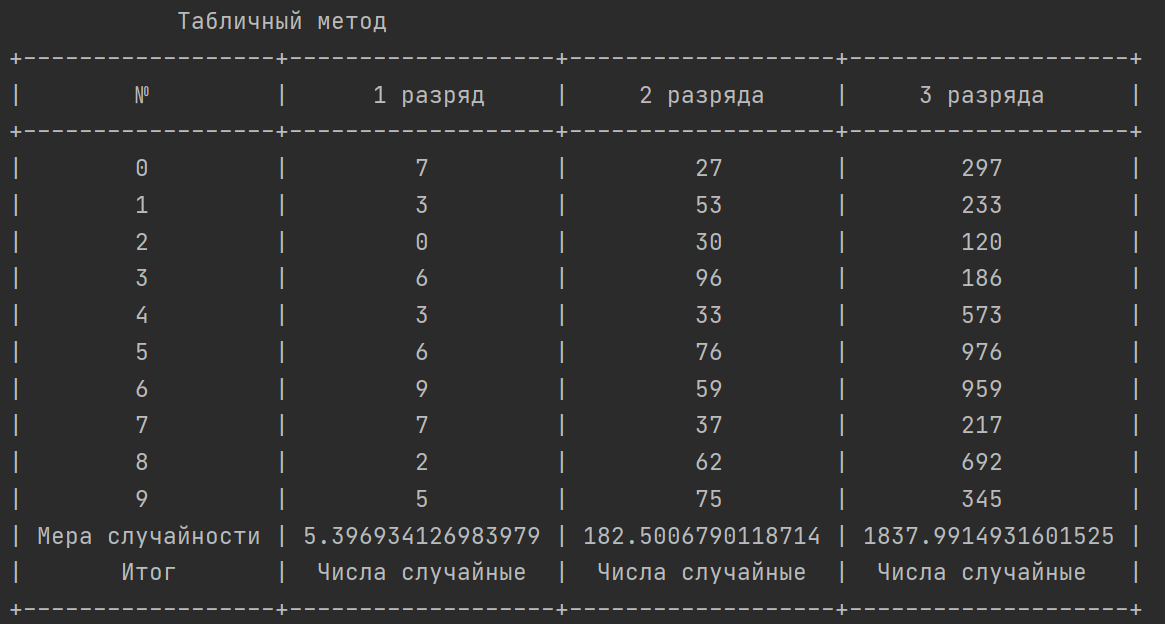
\includegraphics[scale=0.85]{pictures/res_table.png}
			\caption{Результаты расчетов для табличного метода}
			\label{pic:1}}
	\end{center}
\end{figure}

\begin{figure}[h]
	\begin{center}
		{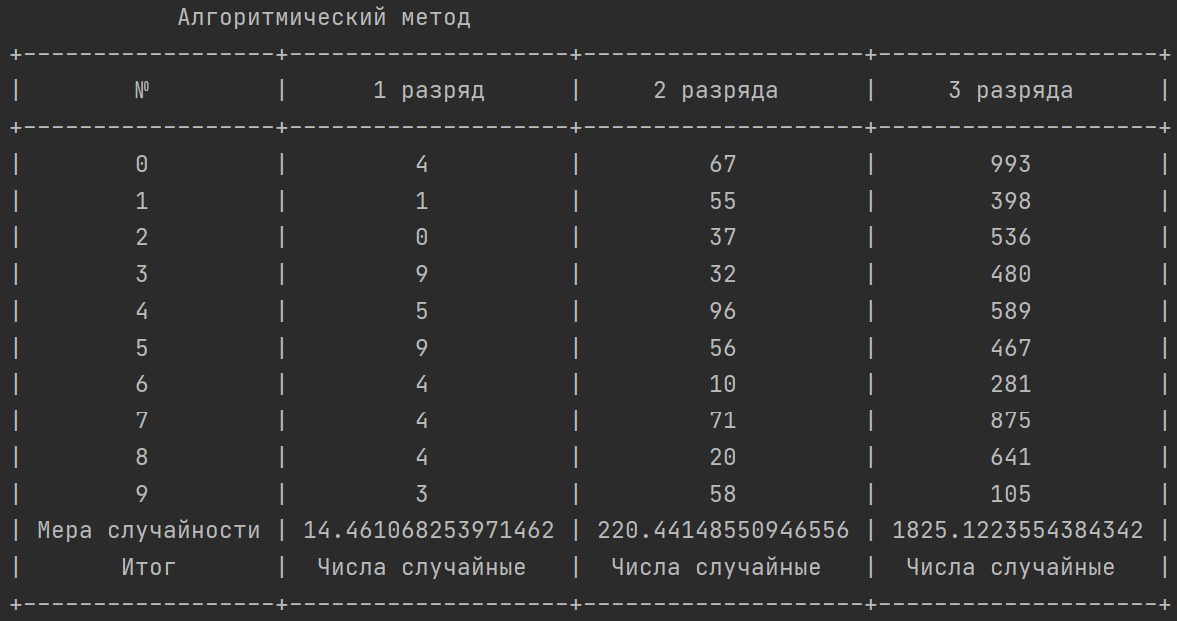
\includegraphics[scale=0.85]{pictures/res_alg.png}
			\caption{Результаты расчетов для алгоритмического метода}
			\label{pic:2}}
	\end{center}
\end{figure}

\newpage
Затем критерий <<случайности>> тестируется на предельных значениях: когда последовательность монотонно возрастает или убывает, состоит из периодечски повторяющихся элементов. Результаты тестирования приведены на рисунке \ref{pic:3}.
\begin{figure}[h]
	\begin{center}
		{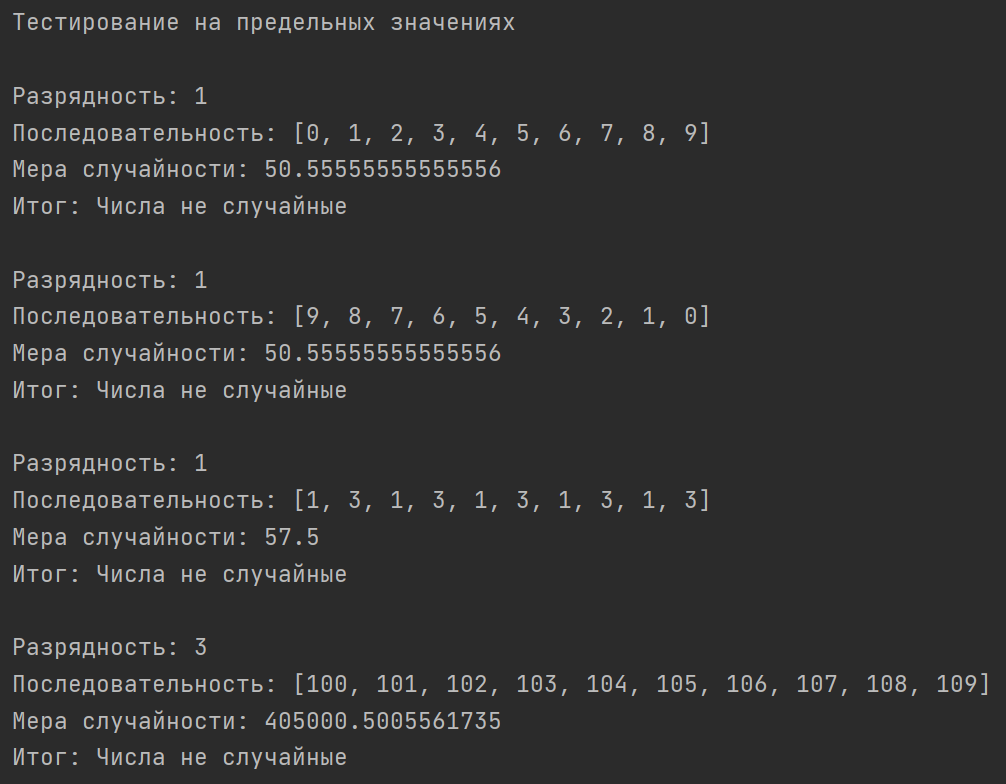
\includegraphics[scale=0.85]{pictures/res_limit.png}
			\caption{Результаты тестирования критерия}
			\label{pic:3}}
	\end{center}
\end{figure}


\newpage
Затем пользователю предлагается ввести собственную последовательность чисел определенной разрядности для проверки ее случайности. Пример работы приведен на рисунке \ref{pic:4}
\begin{figure}[h]
	\begin{center}
		{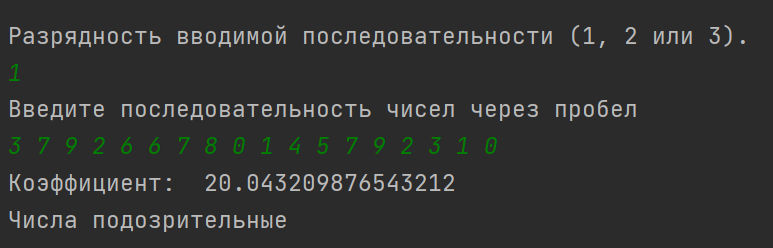
\includegraphics[scale=1]{pictures/res_user.png}
			\caption{Пример обработки пользовательской последовательности}
			\label{pic:4}}
	\end{center}
\end{figure}



\section{Код программы}
Код основной программы, котрая инициирует генерацию последовательностей, рассчитывает критерии и выводит результаты, приведен в листинге \ref{lst:list1} (используемый язык -- Python).

\begin{lstlisting}[caption = {Код основной программы}, label=lst:list1]
from prettytable import PrettyTable
from RandomClass import Random
from math import sqrt

N_RANDOMS = 100000
eps = 1e-6
N_OUTPUT = 10

numbers_limits = {1: [0, 10], 2: [10, 99], 3: [100, 999]}


def hi2_quantiles_for_v(v, ps=(1, 5, 10, 90, 95, 99)):
	return {xp: v + (sqrt(2 * v) * xp) + (2 * (xp ** 2) / 3) - (2 / 3) for xp in ps}


hi2_quantiles = {
	# 1 цифра -> возможные числа [0; 9] -> возможно 19 разниц [-9; 9] (10 чисел)
	1: {1: 2.088, 5: 3.325, 10: 4.158, 90: 14.684, 95: 16.919, 99: 21.666},
	# 2 цифры ->возможные числа [10; 99] -> возможно 179 разниц [-89; 89] (90 чисел)
	2: hi2_quantiles_for_v(89),
	# 3 цифры ->возможные числа [100; 999] -> возможно 1799 разниц [-899; 899] (900 чисел)
	3: hi2_quantiles_for_v(899),
}

def random_from_table():
	with open('random_ints.txt') as file:
		lines = file.readlines()

	numbers = list()
	for line in lines:
		numbers.extend(list(map(int, line.strip().split())))
	numbers = numbers[:N_RANDOMS]
	
	one = [number % 10 for number in numbers]
	two = [10 + number % 90 for number in numbers]
	three = [100 + number % 900 for number in numbers]
	
	return one, two, three


def random_from_alg():
	random = Random(2)
	one = [random.randint(*numbers_limits[1]) for _ in range(N_RANDOMS)]
	two = [random.randint(*numbers_limits[2]) for _ in range(N_RANDOMS)]
	three = [random.randint(*numbers_limits[3]) for _ in range(N_RANDOMS)]
	return one, two, three


def calc_coef(random_numbers, start_random, end_random):
	if start_random != 0:
		end_random += 1
	min_dif = start_random - end_random + 1
	max_dif = end_random - start_random - 1
	
	possible_differences = list(range(min_dif, max_dif + 1))
	probabilities_of_differences = {
		difference: (end_random - start_random - abs(difference)) / ((end_random - start_random) ** 2)
		for difference in possible_differences
	}
	
	n_differences = len(random_numbers) // 2
	differences = [random_numbers[2 * i + 1] - random_numbers[2 * i] for i in range(n_differences)]
	differences_counts = {difference: differences.count(difference) for difference in possible_differences}
	
	if sum(differences_counts.values()) != len(differences) or \
	abs(sum(probabilities_of_differences.values()) - 1) > eps:
		print(sum(differences_counts.values()))
		print(sum(probabilities_of_differences.values()))
		raise ValueError
	
	V = 0
	for difference in differences_counts.keys():
		V += (differences_counts[difference] ** 2) / probabilities_of_differences[difference]
	V = (V / n_differences) - n_differences
	return V


def analyze_coef(counted_coef, digits_amount):
	if counted_coef < hi2_quantiles[digits_amount][1] or counted_coef > hi2_quantiles[digits_amount][99]:
		return "Числа не случайные"
	elif hi2_quantiles[digits_amount][5] < counted_coef < hi2_quantiles[digits_amount][95]:
		return "Числа случайные"
	else:
		return "Числа подозрительные"


def check_limit_values():
	tests = [
	[1, list(range(10))],
	[1, list(range(9, -1, -1))],
	[1, [1, 3, 1, 3, 1, 3, 1, 3, 1, 3]],
	[3, list(range(100, 1000))],
	]
	print('\n\n\nТестирование на предельных значениях')
	for digits, arr in tests:
		print()
		print(f'Разрядность: {digits}')
		print(f'Последовательность: {arr[:min(len(arr), N_OUTPUT)]}')
		coef = calc_coef(arr, *numbers_limits[digits])
		print(f'Мера случайности: {coef}')
		print(f'Итог: {analyze_coef(coef, digits)}')


def main():
	indexes = [i for i in range(N_OUTPUT)]
	
	for alg, alg_name in [[random_from_table, 'Табличный метод'], [random_from_alg, 'Алгоритмический метод']]:
		res_table = PrettyTable()
		one, two, three = alg()
		res_table.add_column("№", indexes + ['Мера случайности', 'Итог'])
		
		one_coef = calc_coef(one, *numbers_limits[1])
		two_coef = calc_coef(two, *numbers_limits[2])
		three_coef = calc_coef(three, *numbers_limits[3])
		res_table.add_column('1 разряд', one[:N_OUTPUT] + [one_coef, analyze_coef(one_coef, 1)])
		res_table.add_column('2 разряда', two[:N_OUTPUT] + [two_coef, analyze_coef(two_coef, 2)])
		res_table.add_column('3 разряда', three[:N_OUTPUT] + [three_coef, analyze_coef(three_coef, 3)])
		
		print(f"\t\t\t{alg_name}")
		print(res_table)
	
	check_limit_values()
	
	print("\n\n\n")
	digits = int(input("Разрядность вводимой последовательности (1, 2 или 3).\n"))
	print("Введите последовательность чисел через пробел")
	arr = list(map(int, input().split()))
	coef = calc_coef(arr, *numbers_limits[digits])
	print("Коэффициент: ", coef)
	print(analyze_coef(coef, digits))


if __name__ == '__main__':
	main()

\end{lstlisting}


Класс Random, реализующий алгоритм вихря Мерсенна, приведен в листинге \ref{lst:list2}.

\begin{lstlisting}[caption = {Класс Random, реализующий алгоритм вихря Мерсенна}, label=lst:list2]

# MT19937, 32-битный генератор MT
class Random():
	def __init__(self, c_seed=0):
		# Параметры n и r выбраны так, что характеристический многочлен примитивный или
		# (nw — r) (число клеток в регистре сдвига, пространство состояний) равна числу Мерсенна 19937
		self.w = 32  # размер слова -- 32 бит
		self.n = 624  # число элементов в регистре сдвига
		self.r = 31  # количество младших бит
		self.m = 397
		
		# Параметры закалки подобраны так, что мы можем получить хорошее равномерное распределение.
		self.l = 18
		self.s = 7
		self.t = 15
		self.u = 11
		self.a = 0x9908B0DF
		self.b = 0x9D2C5680
		self.c = 0xEFC60000
		
		self.f = 1812433253
		
		# Массив для хранения состояний генератора
		self.MT = [0 for _ in range(self.n)]
		self.lower_mask = 0x7FFFFFFF  # битовая маска младших r бит,
		self.upper_mask = 0x80000000  # битовая маска старших w-r бит
		
		# Инициализация
		self.index = self.n + 1
		self.seed(c_seed)
	
	def seed(self, num):
		"""
		Начальное заполнение матрицы состояний
		"""
		self.MT[0] = num
		for i in range(1, self.n):
			temp = self.f * (self.MT[i-1] ^ (self.MT[i-1] >> (self.w-2))) + i
			self.MT[i] = temp & 0xffffffff
	
	def twist(self):
		"""
		Генерация следующих n значений из последовательности x_i
		"""
		for i in range(self.n):
			# Шаг 2. Вычисление (xiu | xi+1l)
			x = (self.MT[i] & self.upper_mask) + \
			(self.MT[(i+1) % self.n] & self.lower_mask)
			# Шаг 3. Вычисление значения следующего элемента последовательности по
			# рекуррентному выражению
			xA = x >> 1
			if (x % 2) != 0:
				xA = xA ^ self.a
			self.MT[i] = self.MT[(i + self.m) % self.n] ^ xA
		self.index = 0
	
	def extract_number(self):
		"""
		Закалка (на основе MT[index])
		Необработанные последовательности, генерируемые рекурсией, обладают плохим равномерным распределением на больших
		размерностях. Чтобы это исправить, используется метод закалки (англ. tempering), на выходе которого получается
		итоговая псевдослучайная последовательность. Метод заключается в том, что каждое сгенерированное слово
		умножается справа на специальную обратимую матрицу T размера w × w.
		Каждые n чисел вызывается twist
		"""
		if self.index >= self.n:
			self.twist()
		# Шаг 4. Вычисление x[i]T
		y = self.MT[self.index]
		y = y ^ ((y >> self.u) & 0xFFFFFFFF)
		y = y ^ ((y << self.s) & self.b)
		y = y ^ ((y << self.t) & self.c)
		y = y ^ (y >> self.l)
		
		self.index += 1
		return y & 0xffffffff
		
	def random(self):
		""" Равномерное распределение [0,1) """
		return self.extract_number() / 4294967296  # 2^w
		
	def randint(self, a, b):
		""" Случайное целое на отрезке [a,b) """
		n = self.random()
		return int(n / (1 / (b-a)) + a)
\end{lstlisting}

\end{document}